
%(BEGIN_QUESTION)
% Copyright 2011, Tony R. Kuphaldt, released under the Creative Commons Attribution License (v 1.0)
% This means you may do almost anything with this work of mine, so long as you give me proper credit

Denne Siemens S7-200 PLC-en er programmert for å telle antall personer i et rom ved å øke en teller hver gang en person går inn døren, og redusere samme teller når noen går ut samme dør.  De to optiske bryterne aktiveres når deres respektive lysstråle brytes av en person som passerer.  Avstanden mellom bryterne er bare noen få tommer -- betydelig mindre enn bredden på en menneskekropp.  Driftsstatusen er at hver bryter aktiverer PLC-inngangen når lysstrålen brytes:

$$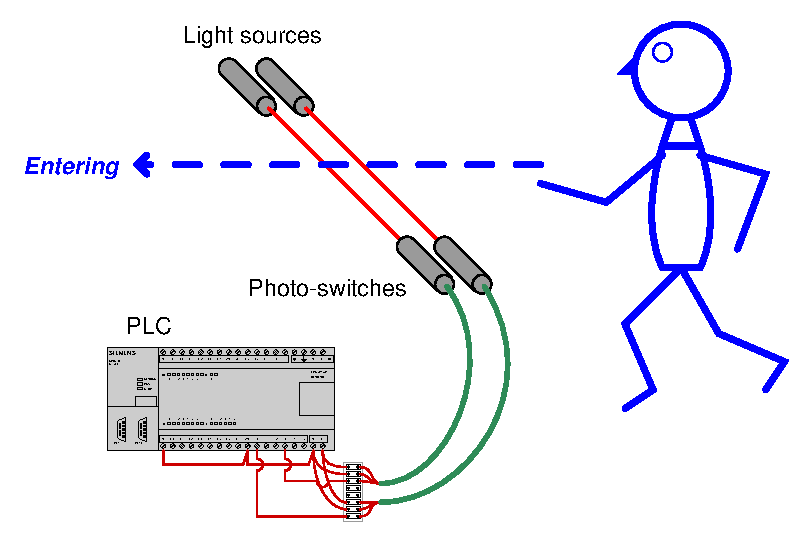
\includegraphics[width=15.5cm]{i00185x01.eps}$$

Studer programmet i denne PLC-en for personelling, og avgjør hvordan det skiller mellom en person som går inn i rommet og en person som går ut:

$$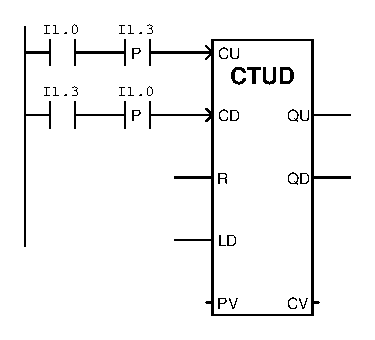
\includegraphics[width=15.5cm]{i00185x02.eps}$$

\vskip 20pt \vbox{\hrule \hbox{\strut \vrule{} {\bf Suggestions for Socratic discussion} \vrule} \hrule}

\begin{itemize}
\item{} Forklar hvordan et \textit{tidsdiagram} for brytertilstandene vil være nyttig i analysen av dette PLC-programmet.
\item{} \textit{Transition}-funksjoner (flankedetektering) implementeres i Allen-Bradley-PLC-er med \textit{one-shot rising} (OSR).  Undersøk hvordan OSR brukes, og hvordan den skiller seg fra ``P''- og ``N''-kontaktene som vises i dette Siemens-programmet.
\item{} Vil systemet fortsatt fungere riktig hvis de optiske sensorene står med større avstand enn bredden på en menneskekropp?  Forklar hvorfor eller hvorfor ikke.
\end{itemize}

\underbar{file i00185}
%(END_QUESTION)





%(BEGIN_ANSWER)

Hint: ``P''-kontaktinstruksjonene er \textit{positive flanke}-instruksjoner, som ``aktiveres'' når tilhørende bit går fra 0 til 1, men går tilbake til ``inaktiv'' når biten blir stående på 0 eller 1.

%(END_ANSWER)





%(BEGIN_NOTES)

Denne tellerinstruksjonen inkrementerer når inngang {\tt I1.3} går fra lav til høy mens inngang {\tt I1.0} allerede er høy (altså i det øyeblikket venstre stråle brytes mens høyre stråle allerede er brutt -- personen går fra høyre mot venstre).

\vskip 10pt

Telleren dekrementerer når inngang {\tt I1.0} går fra lav til høy mens inngang {\tt I1.3} allerede er høy (altså i det øyeblikket høyre stråle brytes mens venstre stråle allerede er brutt -- personen går fra venstre mot høyre).

%INDEX% PLC, ladder logic program analysis and explanation (Siemens S7-200)

%(END_NOTES)

